%%\lstinputlisting[language=Java, firstline=11, lastline=58]{../babyfootClient/clientCore/ClientBabyfoot.java}

\documentclass[a4paper,12pt]{report}
\usepackage[utf8x]{inputenc}
\usepackage[francais]{babel}
\usepackage[top=2cm, bottom=2cm, left=2cm, right=2cm]{geometry}
\usepackage{graphicx}
\usepackage{float}
\usepackage{listings} %Pour le code
\usepackage{ifthen}
\usepackage{color}
\usepackage{textcomp}
\usepackage[babel=true]{csquotes}

\title{Rapport du projet informatique}
\author{Matthieu Denoux - Groupe 1}


\begin{document}
\maketitle
\tableofcontents
\newpage

\part{Analyse du travail effectué}
%%%%%%%%%%%%%%%%%%%%%%%%%%%%%%%%%%
%%                              %%
%%   ------------------------   %%
%%                              %%
%%%%%%%%%%%%%%%%%%%%%%%%%%%%%%%%%%
\chapter{Présentation du sujet}

%%%%%%%%%%%%%%%%%%%%%%%%%%%%%%%%%%
%%   ------------------------   %%
%%%%%%%%%%%%%%%%%%%%%%%%%%%%%%%%%%
\section{Principe général}
\paragraph{}
Le sujet choisi a pour intitulé \textbf{Babyfoot en réseau}. Il s'agit de concevoir un système complet de jeu en réseau.
Le système serait donc séparé en deux parties, un serveur et un client. Chaque joueur pourrait donc se connecter à une partie
n'ayant pas encore commencé et une fois le nombre de joueurs réunis (\emph{2, 3 ou 4}), la partie serait lancée. Il faut donc réaliser à la fois 
le système réseau, l'interface graphique et imaginer un gameplay qui rende le jeu agréable.

%%%%%%%%%%%%%%%%%%%%%%%%%%%%%%%%%%
%%   ------------------------   %%
%%%%%%%%%%%%%%%%%%%%%%%%%%%%%%%%%%
\section{L'interface graphique}
\paragraph{}
Au niveau de l'interface graphique, il faudra réaliser plusieurs fenêtres successives de menus pour parvenir jusqu'au jeu lui-même. Ces fenêtres seront réalisées avec la bibliothèque inclue dans le package standard \textbf{Swing}. J'ai aussi choisi d'utiliser des JFrame et donc de programmer une application à part entière et non une appliquette.
\paragraph{Menu principal}
Un premier menu, dit \emph{menu principal}, permettra de commencer une nouvelle partie en ligne, de rejoindre une partie
déjà en cours, de modifier les quelques options disponibles ou bien de quitter le jeu. Un header unifie les différentes fenêtres, il donnera en plus une certaine identité graphique au jeu avec l'image affichée.
    
    \begin{figure}[H]
	\begin{center}
	
\includegraphics[width=17cm]{pictures/header.png} 
	\end{center}
	\caption{Header du programme, très peu de recherche esthétique, simplement une image de base.}
    \end{figure}
\paragraph{Commencer une partie}
Si l'on commence une nouvelle partie en ligne, on se retrouve dans une \og salle de configuration \fg. Là, il est possible de configurer la partie que l'on souhaite lancer, l'ouvrir à d'autres joueurs, ce qui nous fait arriver dans une \og salle d'attente \fg pour permettre d'attendre que d'autres joueurs rejoignent la partie. Une fois que les équipes sont complètes, on peut lancer le jeu.
\paragraph{Rejoindre une partie}
On peut aussi sélectionner une partie dans la liste des parties déjà commencées, dans la limite des places disponibles. On rejoint alors une \og salle d'attente \fg semblable à celle décrit dans la section précédente où l'on attend que la partie soit complète avant que le meneur, celui qui a créé la partie, ne lance le jeu. C'est le seul qui dispose de cette possibilité.
\paragraph{Déroulement d'une partie}
Le gameplay est entièrement manuel et voit le joueur maître de ses possibilités. Ainsi, les touches \og A \fg, \og Z \fg, \og E \fg, \og R \fg permettent de sélectionner la barre que l'on souhaiterait manier. Le déplacement de la souris vers l'avant et l'arrière permettent quant à elle de déplacer les barres tandis que les deux clics commandent le tir. Je n'ai pas eu le temps de réaliser plusieurs puissances de tir possibles mais cela pourrait consister en une amélioration de la richesse du gameplay. Il est toutefois possible de retenir son tir.
\paragraph{Options}
Un petit menu sera consacré aux options, notamment la sensibilité du déplacement des barres que l'on souhaite utiliser. Un petit démonstrateur a été fait à côté afin de tester cette sensibilité.


%%%%%%%%%%%%%%%%%%%%%%%%%%%%%%%%%%
%%                              %%
%%   ------------------------   %%
%%                              %%
%%%%%%%%%%%%%%%%%%%%%%%%%%%%%%%%%%
\chapter{Analyse de la solution envisagée et mise-à-jour}


%%%%%%%%%%%%%%%%%%%%%%%%%%%%%%%%%%
%%   ------------------------   %%
%%%%%%%%%%%%%%%%%%%%%%%%%%%%%%%%%%
\section{Découpage en modules}
\paragraph{}
J'ai donc découpé le code en deux grandes parties :
\begin{itemize}
    \item Partie client
    \item Partie serveur
\end{itemize}
\begin{figure}[H]
	\begin{center}
	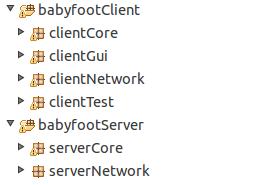
\includegraphics[width=07cm]{pictures/structure.png} 
	\end{center}
	\caption{Structure des fichiers du projet.}
    \end{figure}
Les deux parties (client/serveur) seront elles-mêmes séparées en plusieurs modules.
\begin{itemize}
    \item L'interface graphique (rangée dans /gui) qui sera absente du serveur mais qui consiste en une énorme part du client.
    \item La partie réseau de l'application (rangée dans /network), responsable de l'émission et de la réception des requêtes.
    \item Le c\oe{}ur algorithmique de l'application (rangée dans /core) contenant les classes gérant les matchs, les joueurs, etc. C'est dans le c\oe{}ur du serveur que se font l'ensemble des calculs du jeu.
\end{itemize}
Chaque partie et chaque module comporteront donc plusieurs classes qui se chargeront chacune d'une des tâches du module parent.


%%%%%%%%%%%%%%%%%%%%%%%%%%%%%%%%%%
%%   ------------------------   %%
%%%%%%%%%%%%%%%%%%%%%%%%%%%%%%%%%%
\section{L'interface graphique (client)}
\paragraph{MainFrame.java}
Gère la fenêtre qui englobe tout le reste. On utilisera en fait des JPanel pour modifier le contenu de cette fenêtre. J'empêcherai dans un premier temps de modifier la taille de la fenêtre pour éviter d'avoir des problèmes de dessin du terrain de babyfoot à gérer. Cette classe contient le \textbf{main} du programme. Elle permet d'accéder aux différents éléments : le client récepteur, les informations sur le joueur lui-même, etc.
\paragraph{BPanel.java}
Classe abstraite présentant certaines actions mécaniques quant aux caractéristiques des JPanel utilisés (header, background color, taille, layoutmanager, etc.). Elle contiendra notamment une référence vers l'instance de la fenêtre de type MainFrame La plupart des panels ci-dessous en héritent et peuvent donc accéder à cette classe.
\paragraph{ConnexionPanel.java}
Gère le premier écran affiché à l'ouverture du jeu. On y choisit le pseudonyme que l'on souhaite utiliser dans le reste du jeu et qui s'affichera ensuite sur les écrans lors du contact avec d'autres joueurs. Un message d'erreur est affiché en rouge lorsque le pseudo est déjà utilisé.
\paragraph{MenuPanel.java}
Gère le menu principal affiché après connexion. Contient les boutons qui mèneront vers les principales actions citées plus haut (nouvelle partie, rejoindre, options, quitter).
\paragraph{NewPanel.java}
Lorsque l'on lance une nouvelle partie, on obtient cet écran qui contiendra les principales options nécessaires pour configurer une partie puis l'ouvrir à des joueurs extérieurs. Une fois cette partie ouverte, on aboutit à une \emph{salle d'attente} gérée par WaitingRoomPanel.
\paragraph{ServersPanel.java}
Gère la liste des parties actuellement en recherche de joueurs lorsque l'on cherche à rejoindre une partie. On sélectionne une partie dans cette liste puis on aboutit à une \emph{salle d'attente}. La liste ne se rafraichit pas automatiquement mais un bouton est disponible en bas de page pour le faire.
\paragraph{WaitingRoomPanel.java}
Une fois la partie configurée et ouverte, on aboutit dans cette salle d'attente qui attendra que certaines conditions soient réunies pour permettre au jeu d'être commencé. On peut \emph{aussi} y accéder depuis la partie \emph{rejoindre une partie}. Il est alors possible d'utiliser le chat pour discuter avec les autres joueurs.
\paragraph{GamePanel.java}
La partie à proprement parler. Donc le conteneur du dessin du terrain qui gère les éléments extérieurs, les événements et toute autre interaction avec le reste du code. Inclut la zone de dessin décrite ci-dessous, le panel de chat dans la partie de droite et le panel d'informations sur le match dans celle de gauche.
\paragraph{GameZone.java}
Zone de dessin chargée de représenter le terrain, les joueurs, etc. Fichier assez conséquent puisqu'il contient toute la gestion de l'affichage et des données liées aux actions, déplacements pouvant être effectués par les joueurs sur le jeu. Toutes les informations, les calculs sont effectués par le serveur et envoyées au client qui, via cette classe, se charge de les concrétiser en affichant le jeu. L'affichage est géré par un Thread bien évidemment qui s'occupe de refaire une demande d'actualisation au serveur et affiche les données qu'il possède après la demande, quitte à être en retard d'un tour d'horloge. Ce fichier contient aussi la classe InfoZone qui affiche les informations (score, état) sur le match et donne la possibilité de mettre le jeu en pause et de le supprimer.
\paragraph{ChatPanel.java}
Une partie un peu à part qui est chargée de gérer l'affichage du chat. Celui-ci sera présent à de nombreux endroits : la liste des parties disponibles, la salle d'attente, la création d'une partie et durant le jeu lui-même. Or, tous ces affichages sont centralisés dans cet unique fichier qui centralise ainsi le traitement et l'affichage et permet de réutiliser à plusieurs endroits ces données.
\paragraph{SettingsPanel.java}
Cette classe assez light donne la possibilité de configurer les options du jeu. Je n'ai pas pris le temps d'en configurer beaucoup et il n'est pour l'instant disponible que la modification de sensibilité du jeu. Un démonstrateur a d'ailleurs été inclus à côté des boutons de modification pour tester la sensibilité. Deux boutons sont ensuite possibles : un qui sauvegarde la modification de sensibilité et un autre qui la sauvegarde et revient au menu principal simultanément.
\begin{figure}[H]
	\begin{center}
	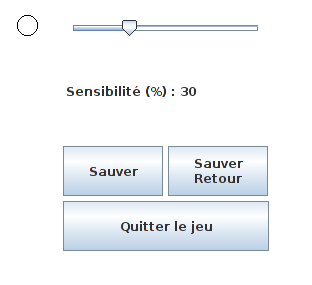
\includegraphics[width=8cm]{pictures/settings.png} 
	\end{center}
	\caption{Image des options de l'écran de configuration avec la présence d'un démonstrateur à gauche pour tester la sensibilité.}
    \end{figure}

%%%%%%%%%%%%%%%%%%%%%%%%%%%%%%%%%%
%%   ------------------------   %%
%%%%%%%%%%%%%%%%%%%%%%%%%%%%%%%%%%
\section{Le réseau}
\subsection{Le principe général}
\paragraph{}
Des messages sont échangés entre le client et le serveur et ce de façon répétée. Il faut donc utiliser des Thread pour gérer l'émission et la réception de données depuis le serveur et un Thread pour gérer la réception côté client. Le serveur se chargera ensuite d'enregistrer les données statiques devant être conservées.
\subsection{La partie client}
\paragraph{ClientBabyfoot.java}
Il s'agit du main du client qui initialise les fenêtres et les différentes classes utilisées.
\begin{quote}
	private static Player player;
    
	private static Chat chat;
    
	private static Client client;
\end{quote}
\paragraph{Client.java}
Cette classe gère la connexion au serveur : il y a en tout trois connexions (une pour le tchat, une pour les joueurs et une pour les données des matchs) afin de pouvoir envoyer plusieurs requêtes simultanément du même client. Toutes les requêtes envoyées sont sous la forme de chaîne de caractères avec l'utilisation d'un caractère spécial, qui est contenu dans une constante de la classe Utils du Core comme séparateur.
\begin{quote}
	private static Socket socketChat;
	
	private static Socket socketPlayer;
	
	private static Socket socketMatch;
	
	private static Socket socketGame;
	
	private ChatClient cc;
	
	private PlayerClient pc;
	
	private MatchClient mc;
	
	private GameClient gc;
	
	private Thread tChat;
	
	private Thread tPlayer;
	
	private Thread tMatch;
	
	private Thread tGame;
\end{quote}
\paragraph{PlayerClient.java}
Gère les différentes actions possibles par et sur les joueurs et les requêtes envoyées au serveur pour pouvoir satisfaire le système (connexion d'un joueur, déconnecter un joueur, ajouter un match, etc.). Elle contient aussi un Thread qui écoute l'entrée de la socket.
\paragraph{MatchClient.java}
Procède de la même façon que PlayerClient pour les matchs, envoie les requêtes au serveur et récupère les données sur la position de la balle, des barres des différents joueurs, etc.
\paragraph{ChatClient.java}
S'occupe de gérer la partie client du tchat : une fois instanciée par le ChatPanel, elle permet d'envoyer des données au serveur et de récupérer la liste des messages disponibles dans le salon. Elle permet aussi de changer de salon, d'afficher la liste des salons et celle des joueurs connectés sur le jeu.
\subsection{La partie serveur}
\begin{figure}[H]
	\begin{center}
	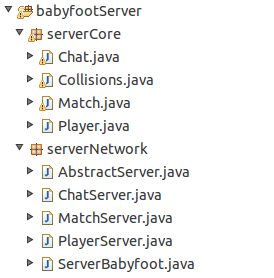
\includegraphics[width=07cm]{pictures/structureserveur.png} 
	\end{center}
	\caption{Structure des fichiers du serveur.}
    \end{figure}
\paragraph{AbstractServer.java}
Classe abstraite qui gère quelques méthodes de base que doivent toutes présenter les classes gérant les serveurs.
\paragraph{ServerBabyfoot.java}
Gère les différentes requêtes et les redirige vers les autres entités du serveur (chat, jeu, etc.). Contient un système de Thread pour pouvoir gérer simultanément ces différentes actions, un Thread général qui gère les requêtes. C'est aussi le main qui lance le serveur.
\begin{quote}
    ServerSocket socketserver = null;
    
	Socket socket = null;
    
	BufferedReader in;
    
	PrintWriter out;
    
	String login;
    
	public static ChatServer tchat;
    
	public static PlayerServer tplayer;
    
	public static MatchServer tmatch;
\end{quote}
\paragraph{PlayerServer.java}
Gère la connexion au serveur d'un des joueurs. L'enregistre dans une liste de joueurs connectés. Peut aussi renvoyer la liste des joueurs connectés actuellement et leur état.
\paragraph{MatchServer.java}
Gère tous les échanges de données sur les matchs. S'occupe ensuite de fournir les informations nécessaires au client sur l'état actuel de la position de la balle par exemple. Nécessitera peut-être, pour des questions de réactivité, d'être multi-threadé.
\paragraph{ChatServer.java}
S'occupe de gérer la partie serveur du tchat : écoute un port, récupère les messages envoyés par des joueurs ainsi que le salon où ils se trouvaient à ce moment là. Les enregistre dans un fichier ou bien dans une base de données (à voir).


%%%%%%%%%%%%%%%%%%%%%%%%%%%%%%%%%%
%%   ------------------------   %%
%%%%%%%%%%%%%%%%%%%%%%%%%%%%%%%%%%
\section{Le c\oe{}ur algorithmique}
\paragraph{Player.java}
Le bloc de base du c\oe{}ur algorithmique est le joueur. Il est instancié par le serveur et a plusieurs attributs : son login, son état actuel (s'il est en train de jouer ou non). Si le joueur est en match, la classe contient aussi les barres qu'il a le droit de déplacer.
\begin{quote}
	private Match match;
    
	private String login;
\end{quote}
\paragraph{Utils.java}
Est une classe abstraite qui gère les fonctions utilitaires comme la mise-en-forme de la date, la mise-en-forme des requêtes, les fonctions de hash utilisées pour vérifier la validité des requêtes, etc. Commune au client et au serveur. Cette classe contient surtout les constantes du programme ainsi que les types créés (enum) pour repérer le côté du joueur, les barres, le statut du match, le type de collision, etc.
\begin{quote}
	public static enum Types { ONEVSONE, TWOVSTWO, ONEVSTWO };
	
	public static enum States { WAITING, FULL, PLAYING, FINISHED };  
	
	public static enum Sides { DOWN, UP };
	
	
	
	public static final int MATCH\_END = 100;
	
	
	
	public static enum Rod { GARDIEN , DEFENSE, MILIEU, ATTAQUE };
	
	public static enum RodStatus { NORMAL, SHOOTING, HOLDING };  
	
	
	
	public static enum CollisionType { SIDES, UPANDDOWN };
	
	
	
	public static final String SEPARATOR = ";";
	
	
	
	public static final int GOAL\_SIZE = 2*100;
	
	public static final int LINE\_STRENGTH = 4;
	
	public static final int GAP\_EDGE = 2*20;
	
	public static final int IMAGE\_PLAYER\_Y = 38;
	
	public static final int IMAGE\_PLAYER\_X = 30;
	
	public static final int MOVE\_STEP = 10;
	
	public static final int BALL\_RADIUS = 15;
	
	
	
	public static final int HEIGHT = 700;
	
	public static final int WIDTH = 900;



	public static final int MAX\_INITIAL\_SPEED = 4;

	

	public static final int GARDIEN\_POSITION = GAP\_EDGE+30;

	public static final int DEFENSE\_POSITION = GAP\_EDGE+30+100;

	public static final int MILIEU\_POSITION = (WIDTH-LINE\_STRENGTH)/2-70;

	public static final int ATTAQUE\_POSITION = WIDTH-Utils.LINE\_STRENGTH-Utils.GAP\_EDGE-230;
\end{quote}
\paragraph{Match.java}
Contient les données principales pour une partie, notamment l'avancement de la partie, l'état des scores, les joueurs y participant, etc. Sera appelée par le serveur. Cette classe contient aussi toutes les informations sur les données factuelles d'une partie, à savoir la position de la balle, la position des barres, etc. Elle se charge d'effectuer l'ensemble des calculs de déplacements de la balle, comptabilise les buts, met en place les pauses.
\begin{quote}
    private int leftScore;
    
	private int rightScore;
	
	private Types type;
	
	private States state;
	
	
	private Player player1;
	
	private Player player2;
	
	private Player player3;
	
	private Player player4;
	
	
	
	private float ballX;
	
	private float ballY;
	
	private float ballSpeedX;
	
	private float ballSpeedY;
	
	
	private Collisions collisions;



	private boolean noSlow = true;

	

	private boolean pause = false;



	private final int STEP\_X = 2;

	private final int STEP\_Y = 2;

	

	private int status = 0;
\end{quote}

\paragraph{Collisions.java}
Gère tout ce qui touche aux collisions, avec les joueurs ou les bords. C'est là que se situe toute la difficulté de calcul. Elle contient donc des attributs pour la gestion de la balle ainsi qu'une Hashtable à deux niveaux stockant les dernières collisions. L'intérêt de la HashTable est ici clairement qu'elle permet de stocker les temps en fonction de la barre et du côté où est situé le joueur.
\begin{quote}
	private float ballX;
	
	private float ballY;
	
	private float ballSpeedX;
	
	private float ballSpeedY;
	
	
	
	private Hashtable\textless Sides, Hashtable\textless Rod, Long\textgreater\textgreater lastCollision;
\end{quote}
\paragraph{Database.java}
Aucune base de données n'a finalement été utilisée. Le serveur stocke donc ses données dans la RAM puis les supprime lors de sa fermeture. Dans un souci de pérennité et de performances, il serait intéressant de les stocker dans des fichiers textes que l'on puisse ainsi conserver des archives.
%%%%%%%%%%%%%%%%%%%%%%%%%%%%%%%%%%
%%                              %%
%%   ------------------------   %%
%%                              %%
%%%%%%%%%%%%%%%%%%%%%%%%%%%%%%%%%%
\chapter{Échéancier}
\paragraph{Ce qui était prévu}
\begin{enumerate}
    \item \textbf{Fin Décembre} : rédiger l'avant-projet.
    \item \textbf{Début/Mi Janvier} : obtenir la validation et les annotations sur la structure choisie.
    \item \textbf{Fin Janvier} : réaliser la partie graphique du programme et avoir regardé les grandes lignes du développement serveur / bases de données. Avoir mis au point les éléments de base du gameplay (interaction joueur/machine).
    \item \textbf{Fin Février} : développer le serveur et la gestion des différents types de requêtes. Mettre au point le tchat et la gestion des joueurs avec la base de données.
    \item \textbf{Mi Mars} : dresser les liens entre serveur et jeu. Tester.
\end{enumerate}
\paragraph{Ce qui a été fait}
\begin{enumerate}
    \item \textbf{Fin Décembre} : rédiger l'avant-projet.
    \item \textbf{Fin décembre/Début Janvier} : développer la partie réseau et l'architecture de base des requêtes.
    \item \textbf{Fin Janvier} : réalisation de l'interface graphique et des premiers calculs pour la mise-en-place de matchs.
    \item \textbf{Février} : ajout des collisions et corrections des principaux bugs liés à la gestion des joueurs, matchs et chat.
    \item \textbf{Mars} : débuguer le reste du programme et ajouter les fonctionnalités supplémentaires nécessaires à un bon fonctionnement.
\end{enumerate}



\part{Évolutions vis-à-vis de l'avant-projet}
\begin{figure}[H]
	\begin{center}
	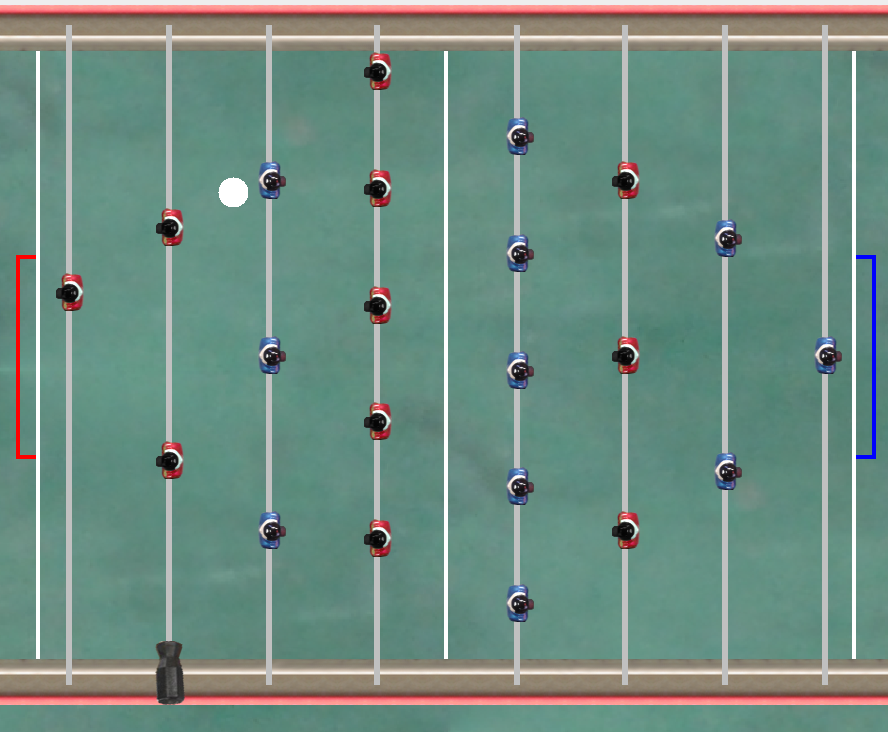
\includegraphics[width=15cm]{pictures/jeu.png} 
	\end{center}
	\caption{Capture d'écran du jeu lui-même et de son aspect.}
    \end{figure}
\paragraph{}
Le projet a été globalement mené à son terme bien qu'il subsiste de nombreux points à améliorer. La programmation de ce projet relativement ambitieux (quelques $5000$ lignes de code jusque là) m'a toutefois permis d'appréhender la mise-en-place d'un réseau en java et le dessin d'une interface graphique. Il aurait pu être intéressant, devant l'envergure que peut prendre un tel projet, de chercher à implanter une stratégie \emph{MVC}, Modèle Vue Controleur, sur le client afin de faciliter l'édition de l'interface graphique et la gestion des données reçues du serveur. C'est ce qui a été partiellement fait : les fichiers Gui sont stockés dans un dossier, les classes gérant les modèles sont faites dans Core et les classes récupérant les données sont dans Network. Néanmoins, la partie logique est en bonne partie gérée dans les vues et non dans les contrôleurs, ce qui gâche toute la logique du MVC.
\paragraph{Au niveau du développement lui-même}
L'\emph{architecture}, bien que réfléchie lors de l'avant-projet, n'est peut-être pas suffisamment stable pour supporter une plus grande charge des clients. Les requêtes peuvent se télescoper, arriver au mauvais client, être redirigée vers le mauvais serveur et des accès simultanés peuvent mal modifier les mêmes informations. L'\emph{interface graphique} doit pouvoir être redessinée, d'abord par souci esthétique et ensuite afin d'intégrer la possibilité pour l'utilisateur de la redimensionner, pour l'adapter à un écran de tablette par exemple.
\paragraph{Pour ce qui est de la structure}
J'ai rajouté quelques classes au projet initial mais toutes n'ont pas été mentionnées ci-dessus car certaines ne sont parfois que des classes implantant l'interface Runnable et initiant des Thread. Globalement, la structure est restée la même, en séparant toutefois bien client et serveur néanmoins, afin de laisser la possibilité que le serveur soit lancé sur une machine indépendante tandis que le client est distribué.
\paragraph{Pour ce qui est du code}
J'ai essayé d'utiliser le plus souvent possible des variables de type \emph{enumerate} afin de rendre plus facile la lecture du code du programme. Il y a relativement peu de commentaires sur l'ensemble du projet car il y a très peu de points très techniques méritant une explication. Le plus difficile est de comprendre l'agencement des classes et leur hiérarchie dans la chaîne aboutissant au jeu.
\paragraph{Choix techniques}
J'ai bien sûr utilisé \textbf{Swing} pour réaliser l'interface graphique : d'abord pour la simple raison que le double-buffering est automatiquement utilisé par Swing, ensuite parce que la structure d'une fenêtre est beaucoup plus souple en ce qui concerne la réalisation de quelque chose d'un peu plus complet. En ce qui concerne le système réseau, j'ai tout simplement utilisé des sockets ainsi qu'elles sont décrites dans le polycopié du cours d'informatique.

\part{Explications des choix techniques}
%%%%%%%%%%%%%%%%%%%%%%%%%%%%%%%%%%
%%   ------------------------   %%
%%%%%%%%%%%%%%%%%%%%%%%%%%%%%%%%%%
\section{Le réseau}
\paragraph{}
Le réseau est au coeur de mon projet et j'ai donc développé plusieurs Thread en parallèle pour pouvoir gérer plus facilement l'envoi de messages par mon application.
Il a fallu mettre au point une nomenclature des messages afin d'obtenir successivement le type de message envoyé et le domaine qui est atteint, donc la classe effectuant le traitement de la requête, puis le joueur concerné (c'est le login qui est utilisé ici bien qu'un système d'ID aurait pu être mis en place) et enfin les données propres à la requête.
\paragraph{}
De plus, le serveur recevant un grand nombre de requêtes, j'ai séparé le serveur en plusieurs entités afin de faciliter le traitement. On trouve ainsi une classe dédiée entièrement à la gestion du Chat et des requêtes échangées. Il y a aussi un serveur se chargeant de gérer les joueurs et enfin, le plus gros des trois, un serveur s'occupant des requêtes de jeux. Il est assez sollicité puisqu'une requête est envoyée aux 2, 3, 4 clients toutes les 20 ms environ (un peu plus parfois). Ces requêtes peuvent être assez longues puisqu'elles contiennent de nombreuses informations : la position des barres, leur statut (normal, levée, tirant) ce qui représente 16 coordonnées puis les huit barres.
\paragraph{}
L'intervalle de temps entre l'envoi de la requête et la réception est aussi légérement variable et est difficilement quantifiable puisque cela dépend de la charge de l'ordinateur, de la longueur du message et de l'utilisation du client au moment de la réception du message. Il m'a donc fallu faire patienter le client ou le faire utiliser des données \og périmées \fg.
\begin{figure}[H]
	\begin{center}
	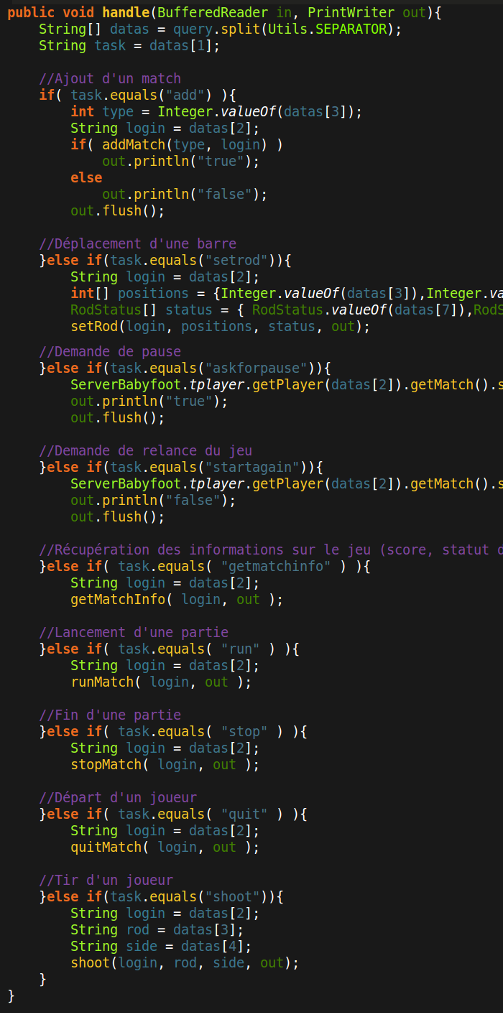
\includegraphics[width=12cm]{pictures/switch.png} 
	\end{center}
	\caption{Sorte de \emph{switch} du projet, permettant de séparer les requêtes selon les différents \og serveurs \fg.}
    \end{figure}
\paragraph{}
Afin d'envoyer un message au serveur, depuis l'interface Gui, par exemple lorsqu'une demande de pause est faite, le schéma est simple. L'interface appelle, via la classe Main, une des classes du Core du client, Player.java par exemple. Cette classe se charge ensuite d'appeler la bonne fonction de la partie Network afin d'envoyer les informations au serveur. Elle récupère par la valeur retournée par la méthode la réponse du serveur et la renvoie à l'interface, en l'ayant traitée au préalable si nécessaire.
\section{La gestion des barres}
\paragraph{}
Un point a été intéressant du point de vue algorithmique, c'est la gestion des barres. Suivant le type de match, un joueur a accès à certaines barres. Par exemple, quand il est seul contre deux joueurs, il a accès à toutes les barres. Par contre, s'il n'est pas seul, le calcul est fait automatiquement selon l'ordre d'arrivée des joueurs dans la partie. Ce qui a été intéressant, c'est de trouver une façon de stocker ces informations. Il fallait ici obtenir une méthode simple pour définir \og l'utilisation \fg des barres, lesquelles sont occupées et lesquelles sont libres. Ce problème est très similaire à un problème d'autorisations et de droits. En effet, a-t-on le droit ou non de bouger les barres ? Comment stocker cette donnée ?
\paragraph{}
Pour cela, ma technique a été très simple, c'est d'utiliser la notation pour binaire et associer à chaque bit une autorisation particulière. Je code ici les autorisations sur quatre bits, chacun représentant deux barres, d'un côté ou d'un autre. Ainsi, les deux premiers bits (valeurs correspondant à \(2^0\) et \(2^1\)) correspondent aux barres du bas et les deux autres à celles du haut. Lorsque le statut des barres est actualisé, \emph{i.e. } qu'un joueur entre dans la partie, cet entier est testé pour situer dans quel cas se situe le jeu et où des barres sont disponibles puis l'entier d'utilisation est mis à jour en ajoutant 1, 2, 3, 4, etc. pour signifier quelles barres va prendre le joueur. De même lorsqu'un joueur quitte la partie, l'entier voit sa valeur soustraite par celle représentant le joueur. On a ainsi une façon simple d'accéder à la possibilité pour un joueur de toucher à une barre puisqu'il s'agit d'utiliser les opérateurs binaires pour tester une autorisation. Ce nombre est stocké par le serveur et est transmis très facilement aux clients qui stockent eux les autorisations dans une Hashtable.
\paragraph{}
Il eut été possible de s'affranchir de toutes ces considérations en réalisant un écran supplémentaire avant le début de la partie où le joueur hôte de la partie aurait tout simplement assigné telle ou telle barre à tel ou tel joueur. La gestion se serait alors faite avec une Hashtable contenant des noms de joueurs par exemple. Il aurait été toutefois intéressant de stocker la même information de \og l'utilisation \fg  des barres afin de vérifier que toutes les barres ont bien été assignées à quelqu'un.
\paragraph{}
La sensibilité d'une barre est aussi très difficile à régler. J'utilise le déplacement relatif de la souris, c'est-à-dire les mouvements \enquote{verticaux} de la souris pour calculer les déplacements des barres. Néanmoins c'est assez difficile car pour une raison que j'ignore, ces déplacements sont asymétriques : la sensibilité est plus grande du haut vers le bas et moins du bas vers le haut. Il faut donc trouver une équation de déplacement qui permette à la fois d'être précis et réactif. L'équation de la différence entre la position après calcul et avant calcul est donnée par la formule ci-dessous :
\begin{quote}
mov = (int)Math.ceil( ( Math.abs( lastKeyY-y )* Utils.getSensibility() / ( 1.+Utils.getSensibility() ) ) );
\end{quote}
\begin{figure}[H]
	\begin{center}
	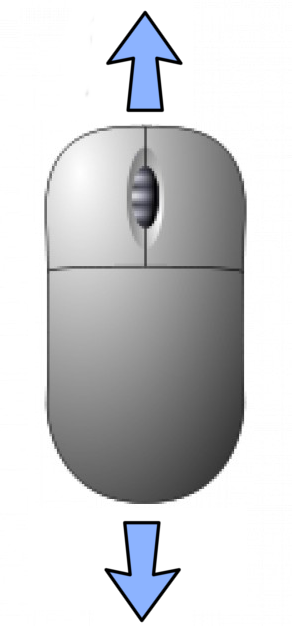
\includegraphics[width=4cm]{pictures/mouse.png} 
	\end{center}
	\caption{Déplacements de la souris servant à mouvoir les barres.}
    \end{figure}
\section{La gestion du jeu}
\paragraph{}
Pour calculer la position de la balle au cours du temps, j'ai utilisé un Thread qui s'actualise toutes les 10ms et qui effectue à chaque tour d'horloge
l'actualisation de la position à partir de la vitesse et des tests de collisions. Les tests de collisions sont calculés à part dans une classe appelée Collision.
Je vérifie ainsi la position de la balle par rapport aux bords et détermine si une collision a eu lieu avec une de ces limites. Une fonction est appelée aussi afin de
déterminer si il n'y a pas eu de contact avec un des joueurs du terrain.
\paragraph{}
La principale difficulté algorithmique vient de cet aspect justement. Parvenir à prévoir les différents comportements de la balle par rapport aux
joueurs. Les coordonnées utilisées par ces calculs diffèrent en plus parfois de celles d'affichage et il faut prendre en compte la taille de l'écran ainsi que les imprécisions dues au caractère discret du calcul. J'ai encore parfois des problèmes de collisions qui se produisent trop tôt, c'est-à-dire que le joueur humain a l'impression qu'elle se cogne contre un objet invisible, ou encore des collisions gérées trop tard auquel cas la balle rentre partiellement dans le joueur en plastique.
\paragraph{}
Une autre difficulté a été de déterminer dans quel sens va la balle après le rebond. En effet, il faut parvenir à placer la balle dans une des quatre zones déterminées par les bissectrices issues des coins du joueur. Si la balle arrive sur les faces avant ou arrière du joueur, elle doit donc voir sa vitesse horizontale changer de sens. Si elle arrive sur les faces de côté, elle doit alors voir sa vitesse verticale changer. Il faut donc calculer la pente de la droite formée par les deux points suivants, le centre de la balle et un des quatre coins du joueur que l'on cherche à étudier, puis la comparer avec la pente de la droite qui marque la séparation. Cela permet ainsi de procéder au rebond.
\paragraph{}
Le problème du caractère discret de ces calculs, c'est que les corrections ne suffisent pas à faire sortir la balle de la zone de collision. Ainsi, malgré le changement de vitesse et la correction effectuée lorsque la balle entre dans une des zones où la collision a lieu, il est possible que la balle reste dans une de ces zones auquel cas, le prochain tour de calcul risque de demander un nouveau changement de vitesse ce qui est bien sûr absurde.
\paragraph{}
Un des derniers défis techniques a été de régler la sensibilité des barres afin de permettre aux joueurs d'avoir à la fois un jeu réactif, confortable, c'est-à-dire où la souris n'a pas besoin de beaucoup bouger, et en même temps quelque chose de suffisamment précis pour pouvoir shooter dans la balle au bon endroit au bon moment.
\paragraph{}
J'ai essayé de mettre au point un amortissement de la vitesse de la balle au cours du jeu. Il est difficile de s'en occuper car, en conservant quelque chose de significatif, il arrive que la balle s'immobilise ce qui est légérement problématique.
\lstset
{
	numberstyle=\footnotesize,
	basicstyle=\ttfamily\footnotesize,
	numbers=left,
	stepnumber=1,
	showstringspaces=false,
	showspaces=false,
	breaklines=true,
	frame=single,
	framexleftmargin=1mm,
	framextopmargin=1mm
}

\definecolor{gray}{gray}{0.5}
\definecolor{green}{rgb}{0,0.5,0}

\lstloadlanguages{Java}
\lstset{language=Java}
\lstset{%
    inputencoding=utf8,
	extendedchars=true,
	literate=%
	{é}{{\'{e}}}1
	{è}{{\`{e}}}1
	{ê}{{\^{e}}}1
	{ë}{{\¨{e}}}1
	{û}{{\^{u}}}1
	{ù}{{\`{u}}}1
	{â}{{\^{a}}}1
	{à}{{\`{a}}}1
	{î}{{\^{i}}}1
	{ô}{{\^{o}}}1
	{ç}{{\c{c}}}1
	{Ç}{{\c{C}}}1
	{É}{{\'{E}}}1
	{Ê}{{\^{E}}}1
	{À}{{\`{A}}}1
	{Â}{{\^{A}}}1
	{Î}{{\^{I}}}1
}
\lstset
{
	language=java,
	basicstyle=\ttfamily\footnotesize,
	stringstyle=\color{red},
	identifierstyle=\color{black}, %
	alsoletter={1234567890},
	otherkeywords={\ , \}, \{},
	keywordstyle=\color{blue},
	upquote=true,
	morecomment=[s]{"""}{"""},
	commentstyle=\color{gray}\slshape
}

\part{Le code partiel du programme}
	\setcounter{chapter}{0}
	\chapter{Client}
	\section{Core}
        \subsection{ClientBabyfoot.java}
            \lstinputlisting[language=Java, firstline=11, lastline=58]{../babyfootClient/clientCore/ClientBabyfoot.java}
        \subsection{Utils.java}
            \lstinputlisting[language=Java, firstline=9, lastline=139]{../babyfootClient/clientCore/Utils.java}
    \section{Gui}
        \subsection{BPanel.java}
            \lstinputlisting[language=Java, firstline=8, lastline=32]{../babyfootClient/clientGui/BPanel.java}
        \subsection{GameZone.java}
            \lstinputlisting[language=Java, firstline=39, lastline=237]{../babyfootClient/clientGui/GameZone.java}
            \lstinputlisting[language=Java, firstline=650, lastline=688]{../babyfootClient/clientGui/GameZone.java}
    \section{Network}
        \subsection{Client.java}
            \lstinputlisting[language=Java, firstline=11, lastline=57]{../babyfootClient/clientNetwork/Client.java}
        \subsection{MatchClient.java}
            \lstinputlisting[language=Java, firstline=15, lastline=340]{../babyfootClient/clientNetwork/MatchClient.java}
    \section{Classe de test}
        \lstinputlisting[language=Java, firstline=12, lastline=53]{../babyfootClient/clientTest/Tester.java}

	\chapter{Serveur}
	\section{Core}
        \subsection{Fonction de tir dans Match.java}
            \lstinputlisting[language=Java, firstline=347, lastline=450]{../babyfootServer/serverCore/Match.java}
        \subsection{Thread de Match.java}
            \lstinputlisting[language=Java, firstline=483, lastline=540]{../babyfootServer/serverCore/Match.java}
        \subsection{Collisions.java}
            \lstinputlisting[language=Java, firstline=16, lastline=214]{../babyfootServer/serverCore/Collisions.java}
    \section{Network}
        \subsection{PlayerServer.java}
            \lstinputlisting[language=Java, firstline=13, lastline=68]{../babyfootServer/serverNetwork/PlayerServer.java}
        \subsection{ServerBabyfoot.java}
            \lstinputlisting[language=Java, firstline=13, lastline=103]{../babyfootServer/serverNetwork/ServerBabyfoot.java}

\end{document}          
